\documentclass[10pt]{beamer}

\usetheme[progressbar=frametitle]{metropolis}
\usepackage{appendixnumberbeamer}

\usepackage{booktabs}
\usepackage[scale=2]{ccicons}
\usepackage{amsmath,amssymb}
\DeclareMathOperator{\E}{\mathbb{E}}
\usepackage{dsfont}
\usepackage{bbold}

\usepackage{pgfplots}
\usepackage{minted}
\usepgfplotslibrary{dateplot}

\usepackage{caption}
\usepackage{subcaption}
\usepackage{changepage}
\usepackage{xspace}
\newcommand{\themename}{\textbf{\textsc{metropolis}}\xspace}

\title{OCaml on the ESP32 chip}
\subtitle{Well typed lightbulbs await}
% \date{\today}
\date{}
\author{Lucas Pluvinage -- ENS Paris}
\institute{
OCaml Workshop -- ICFP 2018
\vspace{1cm}
\begin{figure}
\centering
\hfill
\includegraphics[width=0.3\textwidth]{logo.jpg}
\hfill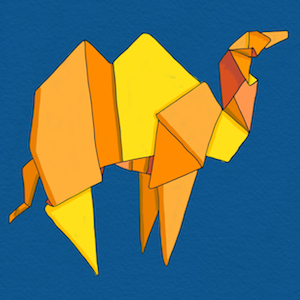
\includegraphics[width=0.15\textwidth]{camel.png}
\hfill
\includegraphics[width=0.3\textwidth]{logo_cam.png}
\end{figure}
}
%\titlegraphic{}

\begin{document}

\maketitle

%\begin{frame}{Sommaire}
%  \setbeamertemplate{section in toc}[sections numbered]
%  \tableofcontents[hideallsubsections]
%\end{frame}
\begin{frame}{Context}
\begin{itemize}[<+->]
\item A language: OCaml
\item A platform: ESP32
\item An application library: Mirage
\end{itemize}
\begin{figure}
\centering
\onslide<1-3>{
\includegraphics[width=.3\textwidth]{ocaml.png}\hfill}
\onslide<2-3>{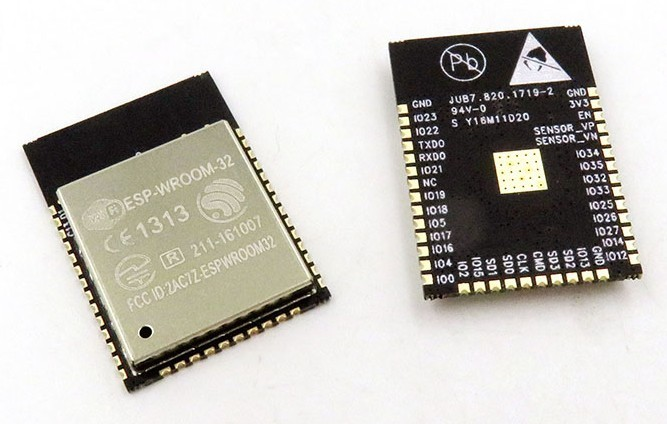
\includegraphics[width=.3\textwidth]{esp32.jpg}\hfill}
\onslide<3>{
\includegraphics[width=.3\textwidth]{mirage.png}}
\end{figure}
\end{frame}

\begin{frame}{ESP32 microcontrollers}
\begin{figure}
\centering
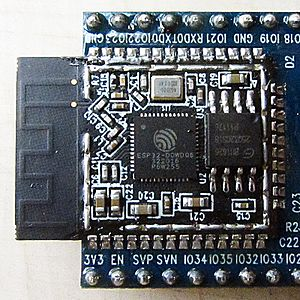
\includegraphics[width=0.3\textwidth]{esp32_photo.jpg}
\hfill
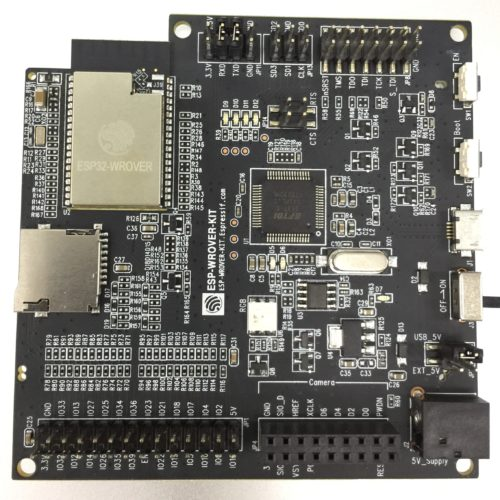
\includegraphics[width=0.3\textwidth]{esp32_wrover.jpg}
\hfill
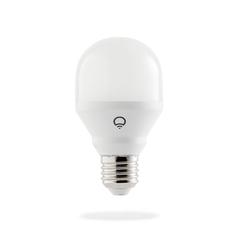
\includegraphics[width=0.3\textwidth]{lightbulb.jpg}
\end{figure}
\end{frame}

\begin{frame}{ESP32 microcontrollers -- hardware}
\begin{figure}
\centering
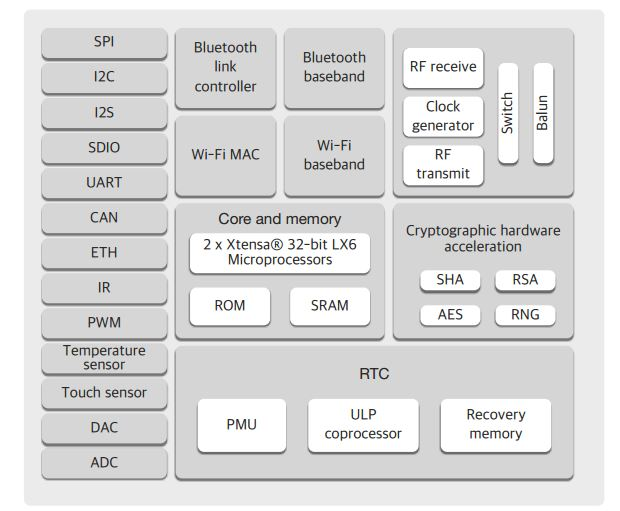
\includegraphics[width=0.95\textwidth]{esp32_features.jpg}
\end{figure}
\end{frame}
\begin{frame}{ESP32 microcontrollers -- software}
\begin{itemize}
\item Espressif IoT Development Framework (ESP-IDF)
\item FreeRTOS (Real-Time Operating System)
\item Written in C -- Xtensa backend for GCC
\item MicroPython port available
\end{itemize}
\pause
\begin{figure}
\centering
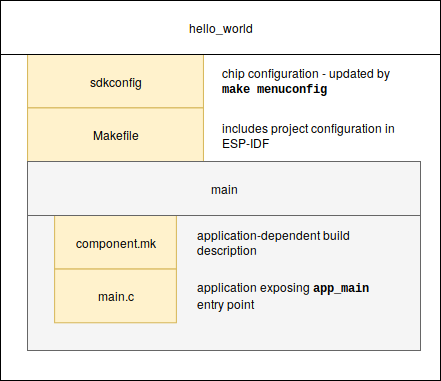
\includegraphics[width=0.6\textwidth]{ESP-IDF.png}
\end{figure}
\end{frame}

\begin{frame}{Mirage unikernel framework}
What is an unikernel ?
\begin{figure}
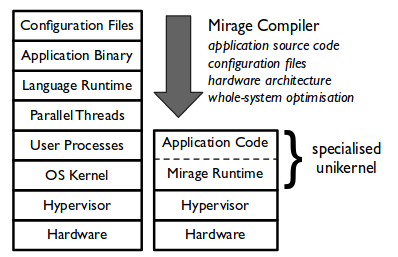
\includegraphics[width=0.95\textwidth]{unikernel.png}
\let\thefootnote\relax\footnote{Picture from \textit{Unikernels: Library Operating Systems for the Cloud}}
\end{figure}
\end{frame}

\section{Time for a demonstration}
\begin{frame}{Time for a demonstration}
\begin{figure}
    \centering
    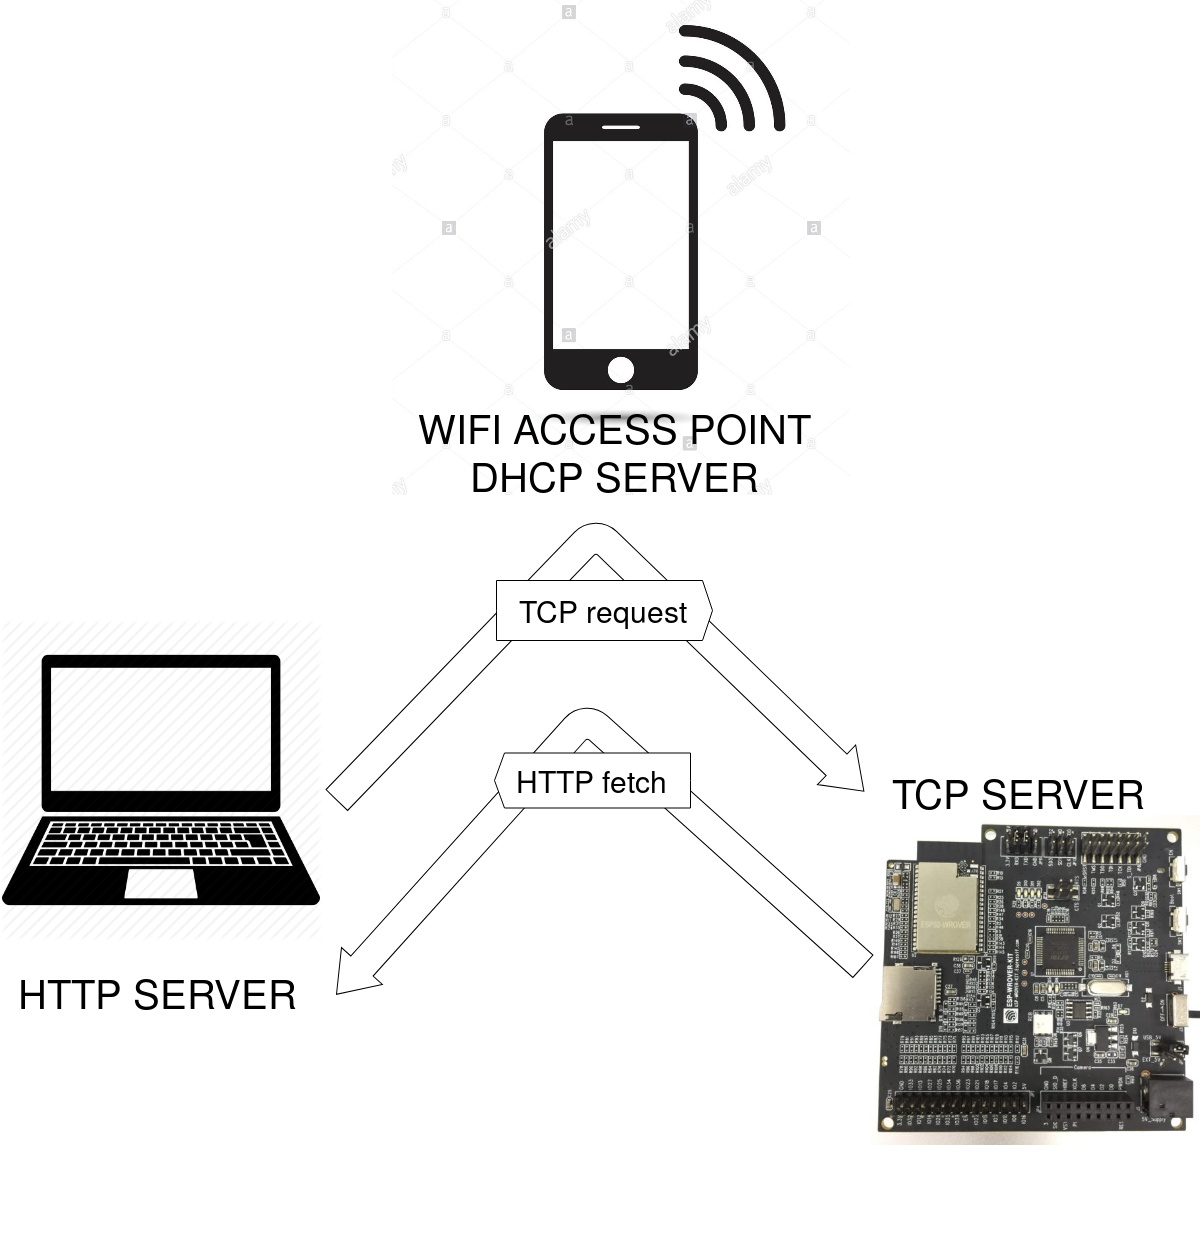
\includegraphics[height=0.95\textheight]{demo.png}
\end{figure}
\end{frame}
\section{Compiling OCaml for ESP32}

\begin{frame}{Compilation paths}
\begin{figure}
\centering
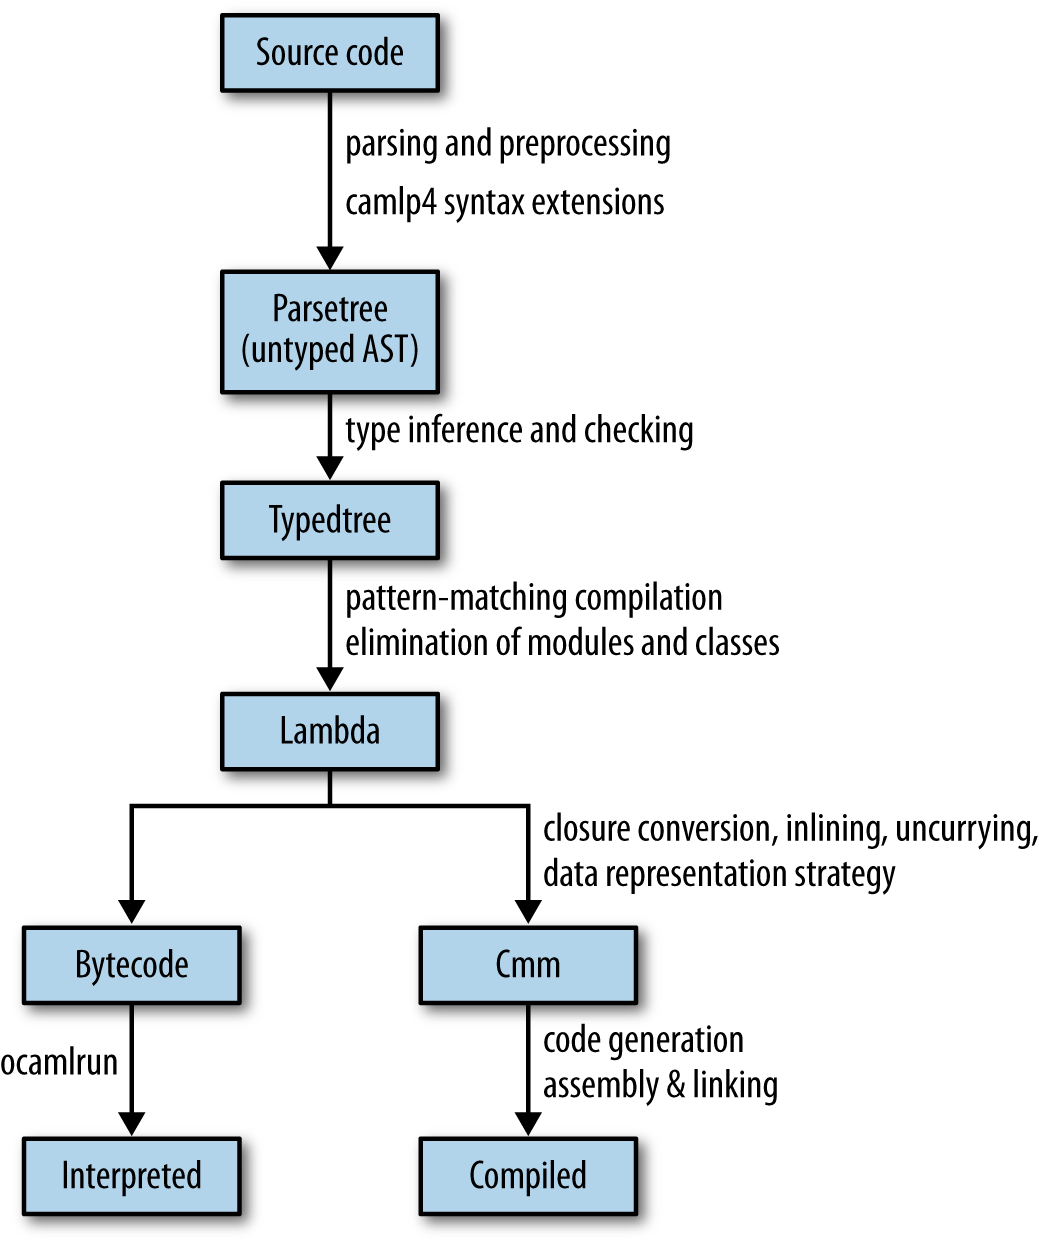
\includegraphics[width=0.6\textwidth]{pipeline}
\let\thefootnote\relax\footnote{Picture from \url{https://dev.realworldocaml.org/compiler-frontend.html}}
\end{figure}
\end{frame}

\begin{frame}{Bytecode execution path on ESP32}
\begin{figure}
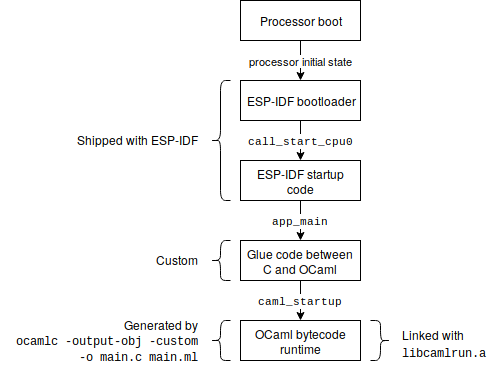
\includegraphics[width=0.95\textwidth]{Bytecode_comp}
\end{figure}
\end{frame}

\begin{frame}{Native compilation support for Xtensa processors}

OCaml compiler backend

\begin{itemize}
\item \texttt{asmcomp/xtensa/} \begin{itemize}
  \item \texttt{proc.ml}: processor and calling conventions
  \item \texttt{arch.ml}: architecture
  \item \texttt{emit.mlp}: assembly emission
  \end{itemize}
\item \texttt{asmrun/xtensa.S} runtime interface between OCaml and C
\end{itemize}

No interference with the OCaml compiler code !
\end{frame}

\begin{frame}{Register windowing and calling conventions}
\begin{figure}
\centering
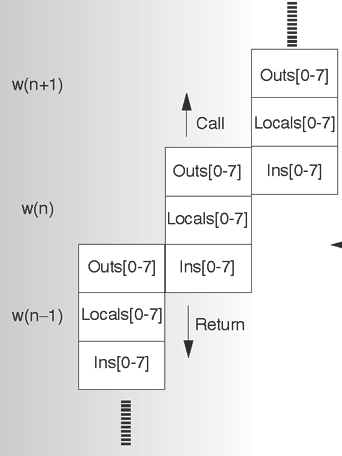
\includegraphics[height=0.9\textheight]{window.png}
\end{figure}
\end{frame}

\begin{frame}{Cross-compiling for ESP32 microcontrollers}
\begin{itemize}
\item Integration with build systems: from a single parameter to more extensive tweaking.
\item Integration with opam:
    \begin{itemize}
        \item OCaml 4.06.0+32bit switch
        \item Cross-compiler in \texttt{[switch root]/esp32-sysroot}
        \item This allows to access both host and target packages.
    \end{itemize}
\item \texttt{opam-cross-esp32}: \large{127} \normalsize packages ported for cross-compilation.
\end{itemize}
\end{frame}

\section{Unikernels for embedded applications}
\begin{frame}{Unikernels and the Mirage project}
\begin{figure}
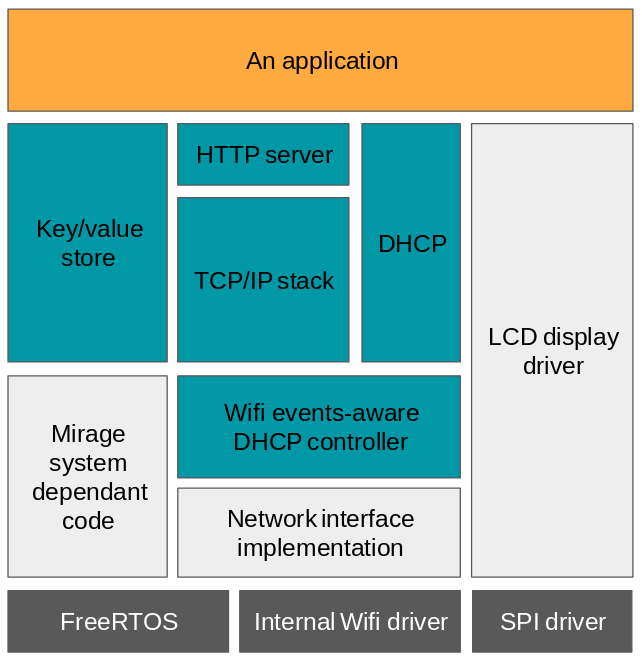
\includegraphics[height=0.95\textheight]{app.png}
\end{figure}
\end{frame}
\begin{frame}{What to you need to build a standalone application ?}
\begin{figure}
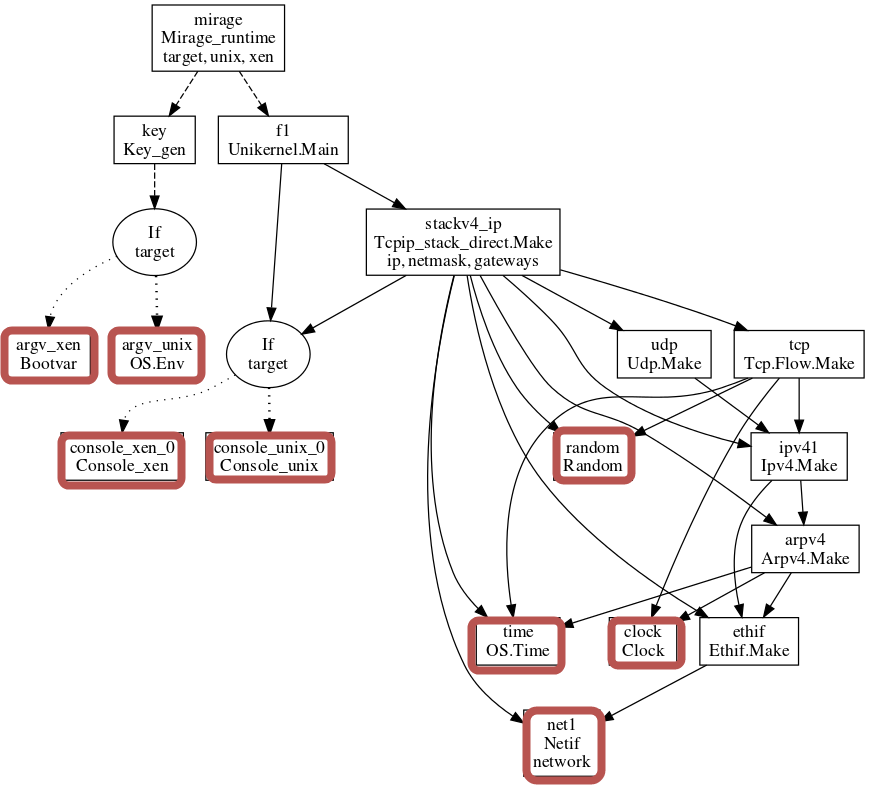
\includegraphics[height=0.95\textheight]{mirage_app.png}
\end{figure}
\end{frame}


\begin{frame}{\texttt{OS.Main.run: unit Lwt.t -> unit}}
\begin{itemize}
\item Collaborative threading with Lwt library: \\ 
\texttt{bind: 'a Lwt.t -> ('a -> 'b Lwt.t) -> 'b Lwt.t} \\ 
\texttt{return: 'a -> a Lwt.t} \\
\texttt{join: unit Lwt.t list -> unit Lwt.t} \\
\texttt{pick: 'a Lwt.t list -> 'a Lwt.t}
\item Timer feature: \\ \texttt{Time.sleep\_ns: int64 -> unit Lwt.t}
\item Event system: \\ \texttt{Event.wait\_for\_event: int -> unit Lwt.t}
\end{itemize}
\end{frame}

\begin{frame}{Porting network features}
\begin{figure}
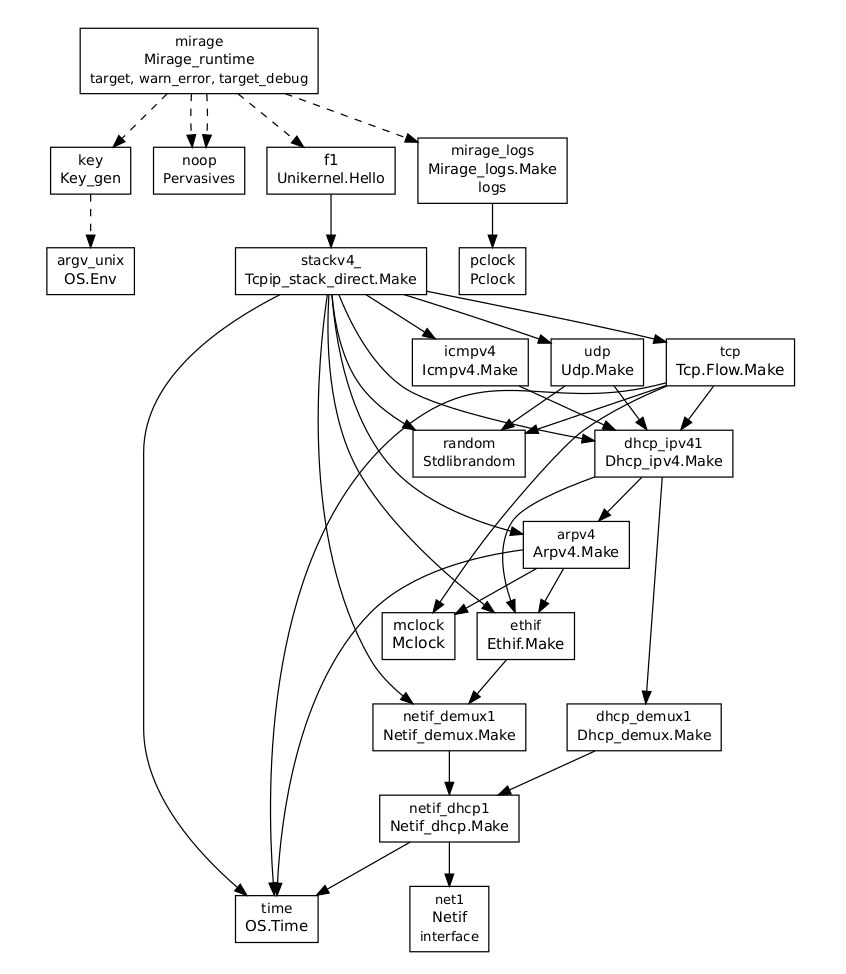
\includegraphics[height=0.95\textheight]{unik.png}
\end{figure}
\end{frame}
\begin{frame}{Porting network features}
\begin{itemize}
    \item Netif: 
    \begin{itemize}
        \item \texttt{write: t -> buffer -> (unit, error) result Lwt.t}
        \item \texttt{listen: t -> (buffer -> unit io) -> (unit, error) result Lwt.t}
        \item \texttt{mac: t -> macaddr}
        \item \texttt{get\_stats\_counters}, \texttt{reset\_stats\_counters}
    \end{itemize}
    \item Netif\_DHCP: input a Netif and outputs a Netif and a DHCP module. Acts as a multiplexer.
\end{itemize}
\end{frame}
\section{Results}
\begin{frame}{Applications}
\begin{itemize}
\item LCD screen control
\item Wifi AP/Station mode/both
\item HTTPS 
\item DHCP
\item DNS
\end{itemize}
\pause
\begin{tabular}{|c||c|c|c|c|c|}
    \hline
    Application & Code & Magic (LTO) & Rodata & Dynamic RAM \\
    \hline
    \hline
    Hello world & 764K & 270K & 151K & 133K \\
    \hline
    AP - DHCP server & 1058K & 405K & 256K & 270K\\
    \hline
    STA - DHCP client & 1217K & 446K & 289K & 215K \\
	\hline
    HTTP fetch & 2366K & 1083K & 622K & 600K \\
    \hline
    HTTPS fetch & 2364K & 1224K & 735K & 700K\\
    \hline
    LCD canvas over HTTP & 2368K & 1038K & 592K & 700K\\
    \hline
\end{tabular}
\pause 
\vfill
LTO is fantastic! See \href{https://github.com/ocaml/ocaml/pull/608}{PR\#608} in \texttt{ocaml/ocaml}
\end{frame}
\begin{frame}{Conclusion}
Main issues
\begin{itemize}
\item<1-4> Memory usage\only<2-4>{: fixed by micro-optimizing assembly generation, taking care of where data is stored, and porting a dead-code elimination patch}
\item<3-4> Bad cross-compilation support
\end{itemize}
\pause[4]
Overview
\begin{itemize}
\item Lot of exploration that resulted in a great proof of concept
\item Opportunity for further research in the field of unikernels for embedded devices
\item Very pleasant team and lab!
\end{itemize}
\end{frame}

\begin{frame}{Resources and conclusion}
\begin{itemize}
\item \texttt{well-typed-lightbulbs} Github organization.
\item \texttt{https://www.lortex.org/esp32/} blog posts.
\end{itemize}
\pause
\begin{figure}
\centering
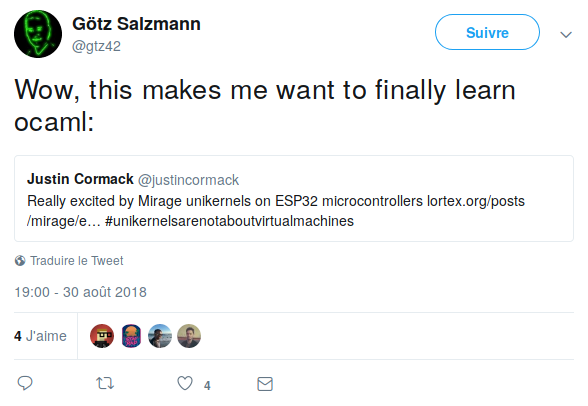
\includegraphics[width=0.8\textwidth]{twit.png}
\end{figure}
\end{frame}
\end{document}
